\documentclass[a4paper, 9pt]{article}

\usepackage[spanish]{babel}
\usepackage{amsmath}
\usepackage{titling}
\usepackage{graphicx}
\usepackage{wrapfig}
\usepackage{color}
\usepackage[]{caption} 
\usepackage{endnotes}
\usepackage{multirow}
\usepackage[utf8]{inputenc}
\renewcommand{\notesname}{}
\renewcommand{\theendnote}{}
\begin{document}
\thispagestyle{empty}
\renewcommand{\contentsname}{Lista de Contenidos}
\renewcommand{\listfigurename}{Lista de Figuras}
\renewcommand{\listtablename}{Lista de Tablas}
\tableofcontents
\listoffigures
\listoftables
\thispagestyle{empty}
\newpage

\begin{abstract}
En esta práctica se trató al mismo material con diferentes medios de enfriamiento, tomando como referencia una de las cuatro muestras de acero 1020, otra se enfrió con agua permitiendo que ésta se temple, la tercera muestra se enfrió en aceite dando lugar al tratamiento térmico de temple en aceite y la última muestra se dejó que se enfríe en el horno, siendo ésta la del enfriamiento más lento, se obtuvo como resultado una muestra recocida, seguidamente se preparó la muestra para realizar el análisis metalográfico y comparar que diferencias existen con respecto a la dureza y micro-estructura que se obtiene en cada tratamiento térmico, se usó lijas de diferentes tamaños empezando por las más gruesas y terminando con las más finas, posteriormente se procedió a realizar el pulido fino con alúmina hasta obtener una superficie translúcida, se concluyo la preparación de la muestra con el ataque químico con nital al $2\%$ y se lo detuvo con metanol, luego se observó por microscopio que cada muestra tiene diferente tamaño de grano y se hizo la medición de dureza obteniendo diferentes valores, siendo el temple con agua la de mayor dureza y el recocido de mayor tenacidad.
\end{abstract}
\section{Teor\'ia}
\setcounter{page}{1}
\captionsetup{font=footnotesize}
\captionsetup[figure]{labelfont=bf,textfont=it}
Los tratamientos térmicos son importante para la obtención final del material a fabricarse, es la fase final de transformación de la materia prima ~\cite{guia}, tiene como objetivo modificar las propiedades del material. Los tratamientos térmicos son diseñados  con enfriamientos y calentamientos establecidos
\begin{wrapfigure}[15]{r}[-2pt]{0.4\textwidth} 
\vspace{-0.8cm}
  \begin{center}
    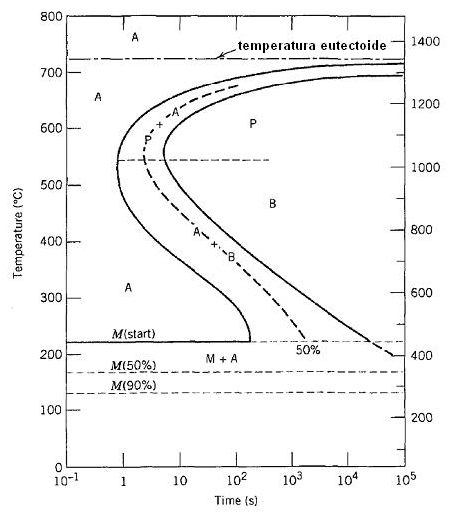
\includegraphics[scale=0.4]{diagrama_TTT.png}
	\vspace{-0.4cm}    
    \caption{Diagrama TTT del Acero}
    \label{diagramaTTT}
  \end{center}
\end{wrapfigure} 
 a determinadas temperaturas y por un tiempo dado de permanencia en una temperatura establecida, para así dar lugar a las transformaciones de fases de la austenita en cualquier otra fase ya sea martensita, perlita o bainita, los diagramas TTT Fig.\ref{diagramaTTT} se determinan por temperatura constante, es decir, fueron determinados de forma experimental al calentar una muestra a una determinada temperatura y la mantenían durante un tiempo hasta completar su transformación en otra fase, otra forma conocida para determinar este tipo de diagramas es por medio de las curvas de enfriamiento continuo, cuyas líneas de transformación se encuentran desplazadas a la derecha con respecto al diagrama TTT Fig.\ref{cct}, este diagrama conocido como CCT por sus siglas en ingles Cooling Curve Transformation es el que mas se asemeja a los procesos usados en la industria, puesto que consiste en la disposición de un cuerpo en medio de enfriamiento de forma continua, dando lugar a una velocidad de enfriamiento constante.
\newpage
Los factores principales que determinan un tratamiento térmico son la transformación de fases durante el calentamiento, el efecto de la tasa de enfriamiento en los cambios estructurales durante el enfriamiento y el efecto del contenido de carbono y de los elementos aleantes.
\\
\begin{wrapfigure}[10]{r}{0.4\textwidth} 
\vspace{-1.4cm}
  \begin{center}
    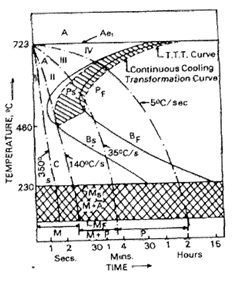
\includegraphics[scale=0.75]{cct.png}%{./Pictures/mainscreen1.png}
	\vspace{-0.45cm}    
    \caption{Diagrama CCT del Acero}
    \label{cct}
  \end{center}
\end{wrapfigure} 
Los diferentes tratamientos térmicos se diferencian por la velocidad de calentamiento, la velocidad de enfriamiento, la atmósfera con la que se desarrolla el tratamiento, entre otros, se conocen diferentes tratamientos térmicos como el recocido, normalizado, temple, revenido y endurecimiento superficial.    
\\
\\
\vspace{0.4cm}
\subsection{Temple}
El temple del acero consiste en el calentamiento hasta la temperatura de austenización y posteriormente el enfriamiento rápido en diferentes medios de disipación de calor como agua, aceite, salmuera o aire ~\cite{libro_guia}, cuando el enfriamiento es rápido, los núcleos no alcanzan a formarse completamente por lo tanto en su microestructura se debe observar una distribución de granos mas pequeños que de una muestra no templada, adicionalmente se produce una distorsión en su estructura cristalina, y como resultado pasa de fcc a tbc, siendo de mayor volumen, dura y fragil.
\\
El fenómeno que tiene lugar en la transformación de fcc a tbc es conocida como la distorsión de Bain~\cite{distorsion_bain}, que consiste en la transformación de dos celdas unitarias en fcc a una sola celda unitaria en tbc, siendo posible incluso calcular el porcentaje volumétrico en que varia, ya que existe  un estudio realizado experimentalmente que relaciona los parámetros de red tanto tbc como fcc con el porcentaje de carbono que contiene el acero Fig.\ref{grafica_parametros_red_distorsion}.
\\
\begin{wrapfigure}[12]{r}{0.4\textwidth} 
\vspace{-0.4cm}
\begin{center}
    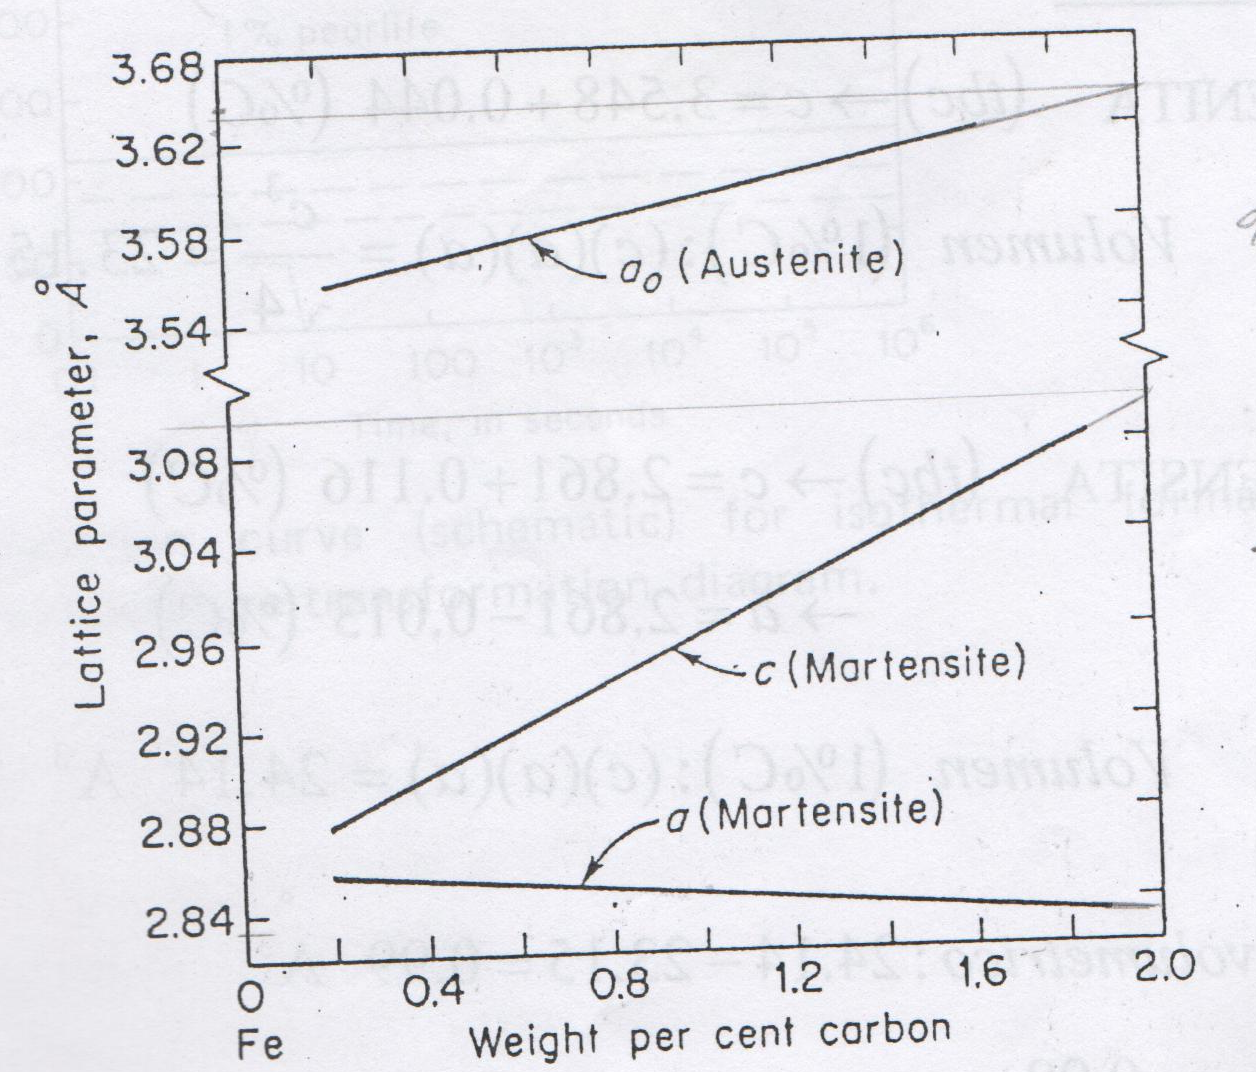
\includegraphics[scale=0.35]{figparametros_de_red.png}
    \vspace{-0.2cm}
     \caption{Variación de parámetros de red Vs. porcentaje de carbono}
    \label{grafica_parametros_red_distorsion}
\end{center}
\end{wrapfigure}
 
Es posible observar en la Fig.\ref{diagramaTTT} que existe un intervalo de velocidades de enfriamiento para las que es posible realizar el temple,siendo la menor la que se encuentra tangente a la nariz perlítica, conocida como la velocidad crítica de temple.
\\
Como resultado del temple se obtiene un porcentaje de martensita de alrededor del $90\%$ conjuntamente con un $10\%$ de austenita retenida que no es posible su transformación en martensita
\subsection{Normalizado}
Este tratamiento térmico consiste en el calentamiento de la muestra hasta una temperatura indicada que depende de sus medidas, y luego se enfría en aire, en el diagrama TTT Fig.\ref{diagrama_normalizado} se observa la curva típica de normalizado, como resultado de este tratamiento térmico se tiene una disminución de la perlita laminar, aumento del contenido de perlita y aumento de dureza, resistencia mecánica y maquinabilidad. 
%incluir figura de normalizado en diagrama ttt
Un fenómeno que ocurre luego de realizar el normalizado es el desplazamiento del punto eutectoide
\begin{wrapfigure}[10]{r}{0.4\textwidth}  
\vspace{-0.8cm}
\begin{center}
    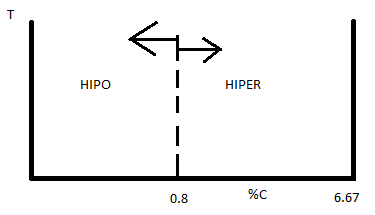
\includegraphics[scale=0.5]{desplaza_eutectoide.png}
     \caption{Desplazamiento del punto eutectoide para aceros hipereutectoides y hipoeutectoides}
    \label{grafica_desplazamiento_punto_eutectoide}
\end{center}
\end{wrapfigure}
ligeramente hacia la derecha o hacia la izquierda dependiendo del tipo de acero, si es un acero hipoeutectoide este punto se desplaza hacia la izquierda del diagrama dando como resultado una disminución del porcentaje de ferrita y un aumento en el porcentaje de perlita, en cambio para aceros hipereutectoides el punto eutectoide se desplaza ligeramente hacia la derecha dando lugar a un aumento de perlita y una disminución de cementita Fig. \ref{grafica_desplazamiento_punto_eutectoide}, como resultado del normalizado se obtiene perlita fina a partir de la perlita gruesa~\cite{normalizado}.
\begin{figure}[h!] 
\centering
    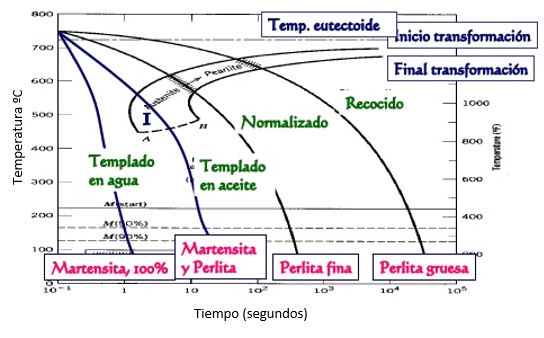
\includegraphics[scale=0.9]{diagrama_normalizado.png}
     \caption{Diferentes tratamientos tèrmicos}
    \label{diagrama_normalizado}
\end{figure}

%incluir grafica de desplazamiento de punto eutectoide
\subsection{Recocido}
Existen tres tipos de recocido conocidos, entre estos se tiene el recocido total, la esferoidización y el alivio de tensiones, teniendo como objetivo la restauración de propiedades luego de haberse realizado el trabajo en frío en la pieza.
\subsubsection{Recocido Total}
Consiste en calentar hasta una temperatura superior a la temperatura crítica inferior, mantener durante un tiempo a dicha temperatura y finalmente se enfría lentamente como en la figura \ref{grafia_ttt_tipico_recocido_total}, dejando que la pieza se enfrié junto con el horno, tiene como objetivo restaurar la microestructura distorsionada y endurecida por el trabajo mecánico en frío por una estructura libre de deformaciones.
\\
\begin{wrapfigure}[11]{r}{0.4\textwidth}  
\hspace{0.25cm}
\begin{picture}(140,90)
\put(0,0){\line(1,5){15}}
\put(0,0){\line(0,1){100}}
\put(0,0){\line(1,0){125}}
\put(15,75){\line(1,0){50}}
\put(65,75){\line(2,-1){45}}
\put(0,60){\line(1,0){5}}
\put(10,60){\line(1,0){5}}
\put(20,60){\line(1,0){5}}
\put(30,60){\line(1,0){5}}
\put(40,60){\line(1,0){5}}
\put(50,60){\line(1,0){5}}
\put(60,60){\line(1,0){5}}
\put(70,60){\line(1,0){5}}
\put(80,60){\line(1,0){5}}
\put(90,60){\line(1,0){5}}
\put(100,60){\line(1,0){5}}
\put(110,60){\line(1,0){5}}
\put(120,60){\line(1,0){5}}
\put(-15,60){\small Tc}
\put(122,-10){\small t}
\end{picture}


\vspace{0.2cm}
\caption{Recocido Total}
\label{grafia_ttt_tipico_recocido_total}
\end{wrapfigure}
El recocido total del acero consta de tres etapas, la primera es la recuperación que tiene lugar en bajas temperaturas, sin modificar su microestructura y su utilidad se presenta al eliminar esfuerzos elásticos, seguidamente se tiene la recristalización siendo esta la etapa más importante presentándose la nucleación de granos sin deformar, esta temperatura de recristalización es aproximadamente el $40\%$ de la temperatura de fusión, aproximadamente $540^{\circ}C$ para el acero, esta temperatura también depende del porcentaje de trabajo en frío que tenga la pieza, ya que se necesitará menor cantidad de energía al ser mayor el porcentaje de trabajado, y finalmente se produce el crecimiento de grano en la etapa final del recocido total, dependiendo de diversos factores como la temperatura de calentamiento y las impurezas presentes.
\\
\subsubsection{Esferoidización}
Es similar al recocido total con la única variante que la temperatura a la que se mantiene luego del calentamiento es una temperatura superior y muy próxima a la tempera crítica inferior.
\\
\subsubsection{Alivio de tensiones}
Se realiza a temperaturas inferiores a la temperatura crítica, es decir, se hace el calentamiento hasta una temperatura inferior a la temperatura crítica, luego se mantiene la temperatura durante un tiempo establecido y al final se enfría dentro del horno.

\subsection{Revenido}
Es un tratamiento térmico que por lo general se realiza después del temple Fig.\ref{temple_revenido}, cuando un acero ha sido tratado por ambas formas, templado y revenido se lo denomina bonificado, este tratamiento tiene como objetivo el disminuir la dureza y aumentar su tenacidad, esto se realiza en diferentes etapas, la primera etapa es el calentamiento hasta una temperatura próxima a los $200^{\circ}C$ dando lugar a la formación de carburos y aumento de dureza, la segunda etapa consiste en calentar hasta $400^{\circ}C$ para transformar la austenita retenida en bainita inferior, la siguiente etapa se calienta hasta $650^{\circ}C$ y como resultado se tiene la transformación de la martensita de tbc a bcc, la disolución de carburos y la formación de troostita, en la cuarta etapa se mantiene a la temperatura crítica inferior, permitiendo la transformación de la cementita en sorbita y la cementita laminar en globular blanda.
\begin{figure}[h!] 
\centering
    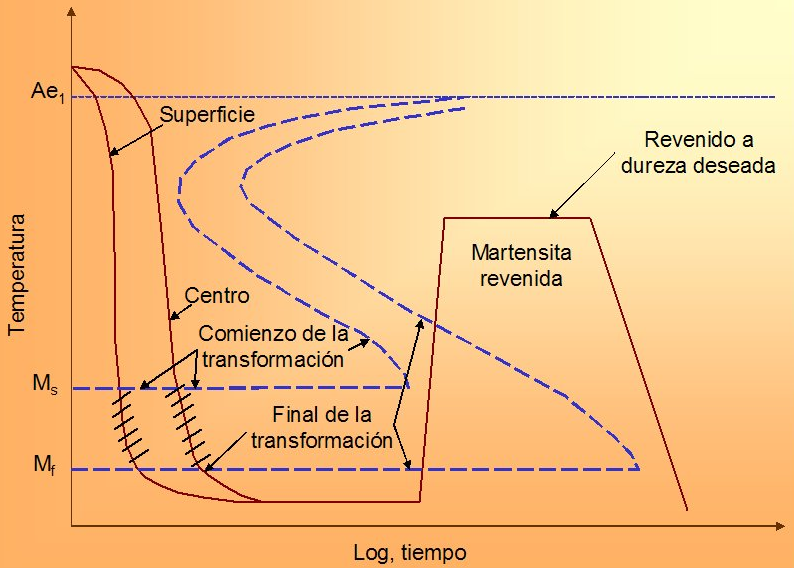
\includegraphics[scale=1.5]{temple_revenido.png}
     \caption{Temple y revenido del acero}
    \label{temple_revenido}
\end{figure}
\
\\
A partir de resultados experimentales obtenidos previamente e investigación bibliográfica ~\cite{dureza}, se conoce que la variación de la dureza es directamente proporcional a la velocidad de enfriamiento, mientras mayor sea la velocidad de enfriamiento mayor sera la medición de dureza, por lo tanto se espera que el acero templado con enfriamiento en agua y hielo sea la pieza con mayor dureza, y la muestra que fue enfriada en el horno sea la de menor dureza, también existe una relación con respecto al tamaño de grano en cada microestructura, puesto que la nucleación es interrumpida sin dejar que crezcan los granos, mayor será la dureza cuando menor sea el tamaño de granos, ya que al ser enfriado de manera brusca no se completa su formación, por lo tanto cuando el enfriamiento es lento sucede lo contrario obteniendo granos de tamaño mayor.  
\\
Existen dos escalas disponibles para realizar la medición de dureza, escala vickers y rockwell, la primera me permite determinar la dureza de cada una de las fases involucradas, ya que es un microdurómetro, en cambio el durómetro rockwell me permite obtener la dureza promedio de una región, en esta práctica se usó el durómetro Rockwell en escala C.
\section{Procedimiento Experimental}
Se tiene cuatro muestras de acero 1020 con 20.5 mm de diámetro, cada una de éstas es sometida a un diferente tratamiento térmico, la primera de las cuatro muestras se la considerará de referencia, ya que a partir de ésta se podrá realizar las comparaciones y las diferencias que existen al ser sometidas a un tratamiento térmico, la segunda será sometida a temple que consiste en calentar hasta la temperatura de austenización aproximadamente $600^{\circ}C$ en el horno, luego se procede a retirar la muestra e inmediatamente se la coloca dentro de un recipiente que contenga agua y hielo Fig.\ref{agua_hielo_foto} para así dar lugar a un enfriamiento rápido durante dos minutos aproximadamente, luego se realiza un procedimiento similar a la tercera muestra pero con diferente medio de enfriamiento, en un envase con aceite durante cuatro minutos de enfriamiento Fig.\ref{practica_aceite}, en cuanto a la preparación de la última muestra ya que tardaría demasiado para llevarse acabo, se nos fue otorgada una muestra que que ya había sido sometida a este tratamiento térmico, en el diagrama TTT de la Fig. \ref{diagrama_normalizado} se puede apreciar las curvas de enfriamiento aproximadas de cada uno de los tratamientos térmicos citados.
\\
Luego se preparó la muestra para su observación en el microscopio óptico, se hizo el pulido grueso con lijas de 220, 320, 400, 600 y 1000 granos por pulgada cuadrada (Marca: Fandelli) Fig. \ref{banco_lijas}, para hacer el desbaste de la superficie a observarse, luego se continuó con el pulido fino untando alúmina en el disco giratorio de la pulidora universal Fig.\ref{pulido_fino} (Marca: Struers), este procedimiento se concluye cuando se observa la superficie translúcida y sin marcas apreciables.
\\
Posteriormente se hizo el ataque químico con nital al $2\%$ para corroer la superficie, ya que está compuesta por diversas fases, cada una reacciona con velocidad diferente, y así poder diferenciarlas en el microscopio en escala de grises, para detener el ataque químico se aplicó metanol sobre la superficie, de esta forma se logró disminuir la velocidad de corrosión hasta anularse completamente.
\\
Luego se midió la dureza de cada una de las muestras, para lograr diferenciar los efectos que ocasionan los tratamientos térmicos empleados, finalmente se realizó las observaciones en el microscopio y con las imágenes obtenidas Sec.\ref{sec:anexos}, se puede inferir en comparaciones entre cada uno de los tratamientos térmicos, y con las mediciones de dureza obtener gráficas de dureza vs. velocidad de enfriamiento.
\\

\section{An\'alisis de Resultados}
A partir de los resultados obtenidos de dureza Tabla.\ref{mediciones_de_dureza} y la tendencia que presentan con respecto al tratamiento térmico Fig.\ref{grafica_tt_dureza}, de forma experimental se obtuvo que la dureza es directamente proporcional a la velocidad de enfriamiento, el temple en agua mejora la resistencia mecánica aumentando la dureza, el temple en aceite ocasiona el mismo efecto pero en menor grado, esto se debe a que la velocidad de enfriamiento es menor que con agua, y como resultado del recocido se obtuvo una menor dureza en comparación a la muestra de referencia, se debe a que su velocidad de enfriamiento es mucho menor y permite la formación de granos grandes.\\
En las imágenes obtenidas por el microscopio óptico Sec.\ref{sec:anexos} se observa las diferentes microestructuras después de aplicar cada uno de los tratamientos térmicos, para el templado en agua y hielo Fig.\ref{micro_temple} se observa un tamaño de grano pequeño, según datos obtenidos previamente ~\cite{u_martensita}, la martensita con un contenido de carbono menor al $0.6\%$ tiene una microestructura denominada martensita en cintas, comparando ambas se puede notar que tienen una microestructura muy similar, por lo tanto es martensita la microestructura luego del temple al agua. Al observar de forma detallada la microestructura del acero templado al aceite Fig.\ref{micro_normalizado} y comparando con imágenes obtenidas previamente ~\cite{u_temple_aceite} se nota una gran similitud en sus estructuras, por lo tanto la microestructura del la muestra de acero templado en aceite es martensita y perlita.\\
En base a datos obtenidos por referencias ~\cite{u_recocido}, comparando con la imagen obtenida Fig.\ref{micro_recocido}, se nota similitud entre las microestructuras, por lo tanto la muestra que fue recocida tiene perlita gruesa en su microestructura.\\
Con respecto a la microestructura obtenida para cada tratamiento térmico, en el temple se obtuvo martensita, en el temple en aceite se obtuvo martensita y bainita, y en el recocido se obtuvo perlita gruesa, todos estos datos concuerdan con la dureza que tiene cada una de las fases involucradas.  
\section{Conclusiones}
Los diagramas CCT y TTT fueron de vital importancia para monitorear cada uno de los tratamientos térmicos analizados y comparados, como resultado se tiene que el temple en agua aumenta en mayor cantidad la dureza que en aceite, en cambio el recocido aumenta su tenacidad, por lo tanto se cumple el triangulo que relaciona la microestructura, las propiedades y los procesos, puesto que al querer variar las propiedades mecánicas fue necesario usar diversos procesos según el objetivo perseguido por el fabricante, si fuese mejorar la resistencia mecánica un proceso requerido seria el temple en agua, si lo que se desea es aumentar la tenacidad, puede ser el recocido el proceso que se necesite, cada proceso se puede diseñar con respecto a que propiedades se quiere variar, para ello primero se recurre a los diagramas de transformación del material en cuestión.

\newpage
\begin{thebibliography}{9}
\bibitem{guia}
  Facultad de Ingeniería Mecánica y Ciencias de la Producción, Área de Materiales, (2016). Laboratorio de Materiales de Ingeniería, Práctica 3: Diagramas TTT y CCT para los tratamientos térmicos del acero.	  
\bibitem{libro_guia}
Serrano, O., (2015). Escuela Superior Politécnica del Litoral., Guayaquil, Guía de Estudio del Curso de Materiales de Ingeniería.
\bibitem{distorsion_bain}
Universidad Politécnica de Valencia, Hipótesis que justifica la transformación de la martensita.,[Fecha de consulta: 23 Julio 2016]. Disponible en: http://www.upv.es/materiales/Fcm/Fcm07/pfcm7\_4\_3.html
\bibitem{normalizado}
Tecnología Industrial. Tratamientos Térmicos. [Fecha de consulta: 23 Julio 2016]. Disponible en: http://www.tecnosefarad.com/wp-content/archivos/bach\_2/materiales/T3\_tratamientos\_termicos.pdf
\bibitem{dureza}
Universidad Autónoma de Madrid, Laboratorio de Materiales, Efectos del enfriamiento, (2004)[Fecha de consulta: 24 Julio 2016]. Disponible en: https://www.uam.es/docencia/labvfmat/labvfmat/practicas/practica4/\\efectos\%20del\%20enfriamiento.htm

\bibitem{u_martensita}
Universidad Autónoma de Madrid, Laboratorio de Materiales, Transformación de Austenita en Martensita, (2004)[Fecha de consulta: 24 Julio 2016]. Disponible en: https://www.uam.es/docencia/labvfmat/labvfmat/practicas/practica4/\\Martensita.htm

\bibitem{u_recocido}
Universidad de Sevilla, Departamento de Ingeniería y Ciencia de los Materiales, Acero de un 0.35\% de C, (2000)[Fecha de consulta: 25 Julio 2016]. Disponible en: http://www.esi2.us.es/IMM2/Pract-html/x-19.html


\bibitem{u_temple_aceite}
Universidad Libre de Colombia, Caracterización Microestructural de un acero AISI-SAE 1045 Tratado Térmicamente en el intervalo crítico [Fecha de consulta: 24 Julio 2016]. Disponible en: http://repository.unilibre.edu.co/bitstream/handle/10901/7839/Caracterizaci\\ \%C3\%B3n\%20Microestructural\%20de\%20un\%20Acero\%20AISISAE\%2010\\45\%20Tratado\%20T\%C3\%A9rmicamente\%20en\%20el\%20Intervalo\%20Inte\\rcr\%C3\%ADtico.pdf?sequence=1

\end{thebibliography}
\newpage
\section{Preguntas Evaluativas}

\subsection{Describir detalladamente la práctica realizada(tiempos, temperaturas, medios de enfriamiento, etc.)}
En esta práctica se realizó dos tratamientos térmicos el temple en agua y en aceite, para ambos casos es necesario medir la temperatura ambiente, aproximadamente $23^{\circ}C$, y la temperatura de las muestras que es igual a la temperatura del horno de $547^{\circ}C$ Fig.\ref{t_de_horno}, para el temple el medio de enfriamiento fue agua y hielo Fig.\ref{agua_hielo_foto} durante dos minutos, para el temple en aceite Fig.\ref{practica_aceite} el enfriamiento fue durante cuatro minutos, para el tratamiento térmico de revenido se tomo como tiempo dos horas de enfriamiento, ya que por falta de tiempo no fue posible realizarse.
\subsection{Describir las fases encontradas en las metalografías de las muestras correspondientes a los diferentes medios de enfriamiento utilizados.}
Se puede observar en la figura \ref{micro_temple} la fase involucrada es martensita, tienen un tamaño de grano más pequeño que la referencia Fig.\ref{micro_referencia}, ésto se debe al medio de enfriamiento ya que no permite la formación de granos grandes, en cuanto al tratamiento de temple en aceite Fig.\ref{micro_normalizado} tiene martensita y perlita como fases involucradas, el tamaño de grano es mayor en comparación al temple, además tienen formas dendríticas, es decir, presentan ramificaciones, finalmente el recocido Fig.\ref{micro_recocido} es el de mayor tamaño de grano de todos los procesos, esto se debe al enfriamiento, ya que es un enfriamiento lento y se observa que tiene granos redondos que se conocen como perlita gruesa, lo que confirma que fue sometido a recocido de esferoidización.

\subsection{Usando el diagrama CCT correspondiente al tipo de acero utilizado en la práctica, trazar las curvas de enfriamiento sugeridas para los tratamientos térmicos realizados, basándose en las fases encontradas en las metalografías obtenidas.}
En figura \ref{diagrama_normalizado} se observa cada uno de los tratamientos térmicos y su producto final, para el temple en agua se obtiene 100\% martensita, para el temple en aceite se obtiene martensita y perlita y para el recocido resulta perlita gruesa.\\

\subsection{Describir las diferentes curvas y regiones encontradas en los diagramas TTT.}
Se observa en la figura \ref{diagramaTTT} las diferentes regiones que conforman un diagrama TTT, los principales puntos a recalcar son la velocidad crítica de temple que es tangente a la nariz perlítica, las líneas de transformación que denotan el tiempo que tarda la austenita en pasar a ser bainita, ferrita o perlita, a temperaturas altas se observa que se transforma en cementita y algo de austenita, a temperaturas próximas a los $600^{\circ}C$ se tiene la cementita y perlita, a temperaturas menores en cambio se obtiene bainita, se observa además que entre los $200^{\circ}C$ y $100^{\circ}C$ se tiene dos fases, martensita y austenita.  
\subsection{Describir y comparar los siguientes tratamientos térmicos:}
\subsubsection{Temple}
Tratamiento térmico que consiste en enfriamiento rápido a partir de la austenita, se caracteriza por modificar las propiedades mecánicas, mejorando su resistencia y dureza a cambio de una disminución de su tenacidad y ductilidad, su estructura metalográfica es de granos más pequeños que antes de temple, de todos lo procesos térmicos citados aquí, es el de mayor dureza.
\subsubsection{Revenido}
Tratamiento térmico que normalmente se lleva a cabo luego del temple, cuando un acero es templado y revenido se conoce como acero bonificado, tiene como objetivo mejorar la ductilidad, ya que luego del temple se tiene baja ductilidad, su microestructura es de granos más grandes, y tiene menor dureza que el templado.
\subsubsection{Recocido}
Consiste en la recuperación de las propiedades mecánicas del material, cuando éste ha sido trabajado en frío, sus propiedades mecánicas depende de las temperaturas de operación de cada etapa del recocido, en esta práctica la muestra recocida tiene menor dureza de todos los tratamientos térmicos.
\subsubsection{Normalizado}
Tiene como objetivo formar perlita fina, mejorando su resistencia mecánica, esto se debe al desplazamiento del punto eutectoide, de todos los tratamientos térmicos al aplicar este se obtiene una dureza promedio, menor que la del templado y mayor que la del recocido.
\subsection{Describir el comportamiento mecánico de aleaciones de Fe-C de acuerdo al contenido de:}
\subsubsection{Ferrita}
Las ferritas se producen a menudo en forma de polvo, con el cual se pueden producir piezas de gran resistencia y dureza, previamente moldeadas por presión y luego calentadas, sin llegar a la temperatura de fusión, dentro de un proceso conocido como sinterización. Mediante este procedimiento se fabrican núcleos para transformadores, inductores$/$bobinas y otros elementos eléctricos o electrónicos.
\subsubsection{Cementita}
La cementita es muy dura, de hecho es el constituyente más duro de los aceros al carbono, con una dureza de 68 HRc. La cementita destaca por ser un constituyente frágil, con alargamiento nulo y muy poca resiliencia. Su temperatura de fusión es de $1227^{\circ}C$. como la cementita es muy dura y frágil no es posible utilizarla para operaciones de laminado o forja debido a su dificultad para ajustarse a las concentraciones de esfuerzos.
\subsubsection{Perlita}
Hay dos tipos de perlita, la perlita fina que es dura y resistente, y la erlita gruesa que es menos dura y más dúctil.
La razón de este comportamiento radica en los fenómenos que ocurren en los límites de fases ($\alpha$ y cementita). En primer lugar, hay un alto grado de adherencia entre las dos fases en el límite. Por lo tanto, la resistencia y la rigidez de la fase cementita restringe la deformación de la fase (ferrita), más blanda, en las regiones adyacentes al límite; es decir, la cementita refuerza a la ferrita. Este grado de reforzamiento es más elevado en la perlita fina porque es mayor la superficie de límites de fases por unidad de volumen del material. Además, los límites de fases sirven de barrera para el movimiento de dislocaciones, del mismo modo que los límites de grano. En la perlita fina y durante la deformación plástica las dislocaciones deben cruzar más límites de fases que en la perlita gruesa. De este modo el mayor reforzamiento y restricción del movimiento de las dislocaciones en la perlita fina se traducen en mayor dureza y resistencia mecánica. La perlita gruesa es más dúctil que la perlita fina a consecuencia de la mayor restricción de la perlita fina a la deformación plástica.
\subsubsection{Bainita}
Es una mezcla entre las fases ferrita y cementita, comúnmente esta formado por una matriz ferrítica y tiene cementita en forma alargada, existen dos formas de bainita, la superior e inferior, se diferencian por la temperatura a la que se obtienen. Los aceros bainíticos son más duros y resistentes que los perlíticos porque tienen una estructura más fina a base de partículas diminutas de cementita en una matriz ferrítica. Por este motivo exhiben una interesante combinación de resistencia y ductilidad.
\subsubsection{Martensita}
Los aceros con microestructura martensítica son los más duros y mecánicamente resistentes, pero también los más frágiles y menos dúctiles. La dureza de estos aceros depende del contenido en carbono; aun así, son más tenaces que los aceros perlíticos. La martensita es una solución sólida sobresaturada de carbono y austenita.

\subsection{Describa cómo y bajo qué condiciones(temperaturas) ocurren las siguientes transformaciones de fase:}
\subsubsection{Transformación de Austenita a Perlita}
Después de calentar la pieza a una temperatura mayor a la temperatura de austenización, se procede al enfriamiento lento, sólo bajo condiciones de enfriamiento muy lento se puede obtener perlita, en este caso se obtiene un tamaño de grano más grande ya que  la nucleación no es interrumpida.
El rango de temperaturas aproximado para una transformación isotérmica  está entre los $500^{\circ}C$ y $700^{\circ}C$.
\subsubsection{Transformación de Austenita a Bainita}
Luego de ser calentado a una temperatura mayor a la de austenización, se enfría hasta una temperatura ligeramente inferior a la nariz perlítica, se mantiene a temperatura constante y se deja expuesta a un enfriamiento lento.
El rango de temperaturas aproximado para su transformación isotérmica está entre los $450^{\circ}C$ y $260^{\circ}C$.
\subsubsection{Transformación de Austenita a Martensita}
La pieza al ser llevada a una temperatura mayor a la temperatura de austenización, aproximadamente $740^{\circ}C$, luego se procede a enfriar de forma severa la pieza con lo que no se permite el crecimiento de granos de forma completa, para la transformación de la austenita en martensita no se requiere tiempo, esto ocurre siempre y cuando la velocidad de enfriamiento sea mayor a la velocidad critica de temple.
El rango de temperaturas aproximado donde coexisten las fases austenita y martensita está entre los $100^{\circ}C$ y $200^{\circ}C$.

\newpage
\section{Anexos} 
\subsection{Determinación de velocidades de enfriamiento}
Para determinar la velocidad de enfriamiento de cada una de las muestras se toma la diferencia entre la temperatura del horno y la temperatura ambiente, y se divide para el tiempo total de enfriamiento, como resultado se tiene;
\renewcommand{\tablename}{Tabla}


\begin{table}[htbp]
\begin{center}
\begin{tabular}{|c|c|c|c|}
\hline
Tratamiento Térmico & Temple Agua & Temple Aceite & Recocido \\
\hline 
T. Ambiente ($^{\circ}C$) & 23 & 23 & 23 \\ 
\hline
T. Muestra ($^{\circ}C$) & 547 & 547 & 547 \\ 
\hline
Tiempo (seg) & 120 & 240 & 7200*\endnote{\hspace{2.35cm} *Tiempo estimado, no realizado en la práctica} \\ 
\hline
V. Enfriamiento & 4.367 & 2.183 & 0.073\\ 
\hline
\end{tabular}
\caption{Datos velocidad de enfriamiento}
\label{velocidad_enfriamiento}
\end{center}
\end{table}
\vspace{-2.3cm}
\theendnotes

	
\subsection{Mediciones de dureza}
Para poder hacerse la comparación es necesario que en todas las muestras se aplique la misma cargar (100kgf) y el mismo identador ($1/16$ in. punta redonda).
\begin{table}[htbp]
\begin{center}
\begin{tabular}{|c|c|c|c|}
\hline
Referencia & Agua+Hielo & Aceite & Recocido \\
\hline 
87.3 & 96.6 & 85.9 & 82.3 \\ 
\hline
87.7 & 97.4 & 85.3 & 83.5 \\ 
\hline
87.6 & 96.9 & 86.3 & 83.8 \\ 
\hline
86.9 & 97.5 & 85.7 & 82.9 \\ 
\hline
87.9 & 97.6 & 85.5 & 82.8 \\ 
\hline
87.4 & 96.9 & 85.7 & 83.4 \\ 
\hline
\end{tabular}
\caption{Mediciones de dureza Rockwell C}
\label{mediciones_de_dureza}
\end{center}
\end{table}

\begin{figure}[h!] 
\centering
    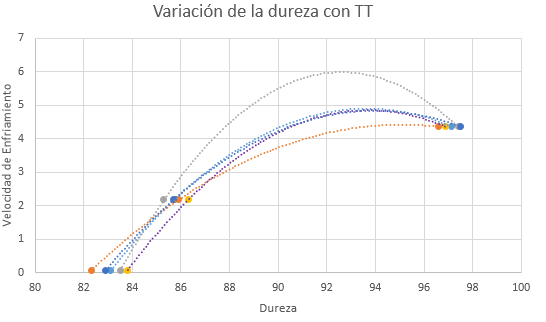
\includegraphics[scale=0.85]{grafica_tt_dureza.png}
     \caption{Variación de la dureza con respecto al tratamiento térmico}
    \label{grafica_tt_dureza}
\end{figure}
\newpage
\subsection{Imágenes obtenidas por el microscopio} \label{sec:anexos}
Imágenes con aumento de 500x.

\begin{figure}[h] % indico que voy a poner una figura y [h] indica que la posición relativa, tambien puedo usar t = top entre otros.

\hfill
\begin{minipage}[t]{.45\textwidth}
\begin{center}
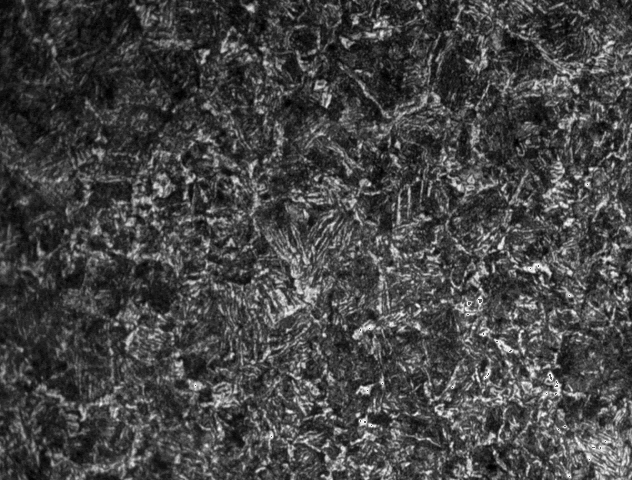
\includegraphics[scale=0.5]{Aceite.jpg}
\caption{Microestructura de temple en aceite}
\label{micro_normalizado}
\end{center}
\end{minipage}
\hfill
\begin{minipage}[t]{.45\textwidth}
\begin{center}
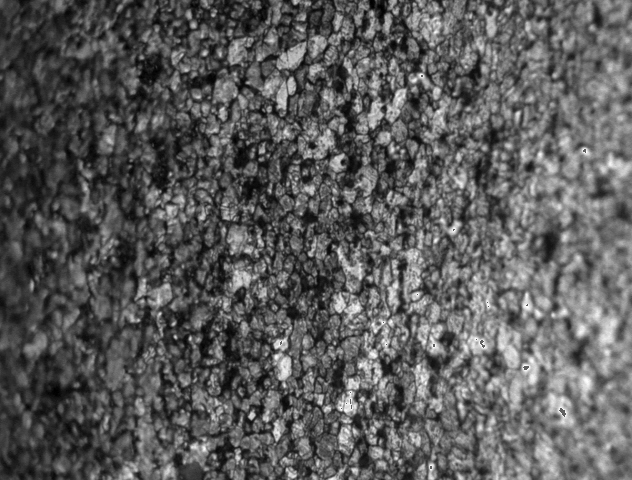
\includegraphics[scale=0.5]{Agua_hielo.jpg}
\caption{Microestructura de temple}
\label{micro_temple}
\end{center}
\end{minipage}
\hfill
\end{figure}

\begin{figure}[h] % indico que voy a poner una figura y [h] indica que la posición relativa, tambien puedo usar t = top entre otros.

\hfill
\begin{minipage}[c]{.45\textwidth}
\begin{center}
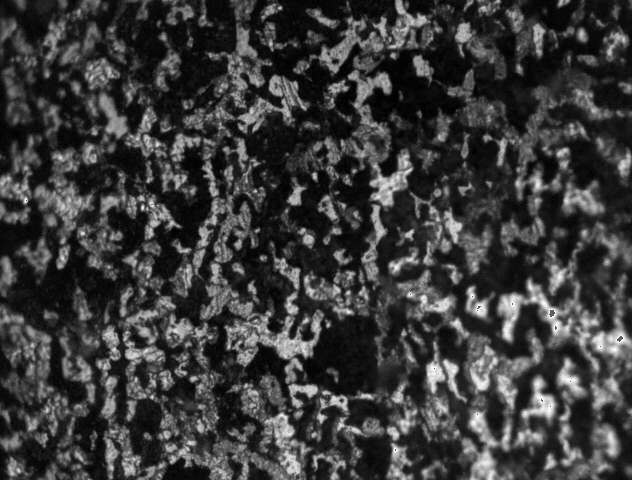
\includegraphics[scale=0.5]{Recocido.jpg}
\caption{Microestructura del recocido}
\label{micro_recocido}
\end{center}
\end{minipage}
\hfill
\begin{minipage}[c]{.45\textwidth}
\begin{center}
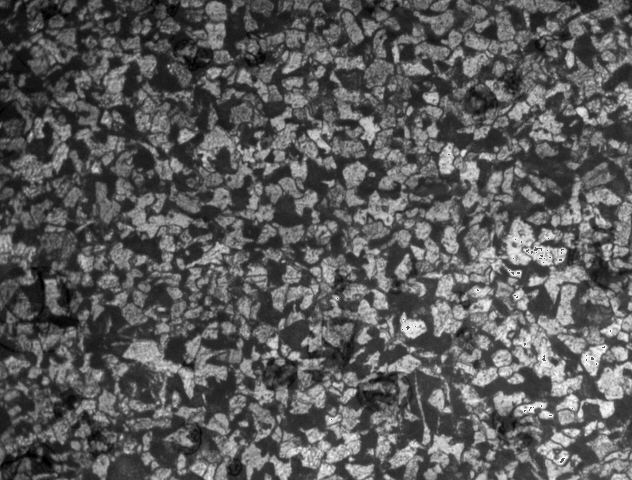
\includegraphics[scale=0.5]{Referencia.jpg}
\caption{Microestructura de la muestra de referencia}
\label{micro_referencia}
\end{center}
\end{minipage}
\hfill
\end{figure}
\newpage
\subsection{Fotos de la practica}

\begin{figure}[h!] % indico que voy a poner una figura y [h] indica que la posición relativa, tambien puedo usar t = top entre otros.

\hfill
\begin{minipage}[t]{.45\textwidth}
\begin{center}
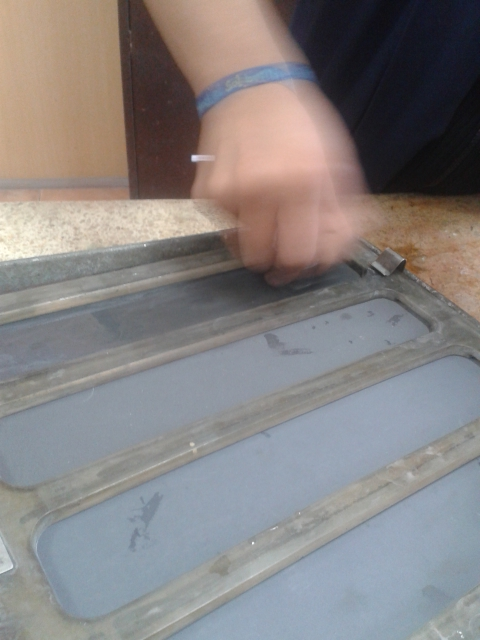
\includegraphics[scale=0.2]{banco_lijas.jpg}
\caption{Banco de lijas}
\label{banco_lijas}
\end{center}
\end{minipage}
\hfill
\begin{minipage}[t]{.45\textwidth}
\begin{center}
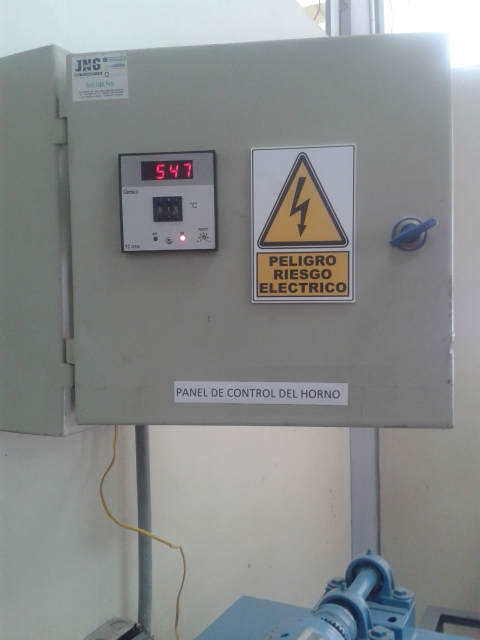
\includegraphics[scale=0.2]{t_de_horno.jpg}
\caption{Temperatura del horno}
\label{t_de_horno}
\end{center}
\end{minipage}
\hfill
\end{figure}

\begin{figure}[h!] % indico que voy a poner una figura y [h] indica que la posición relativa, tambien puedo usar t = top entre otros.

\hfill
\begin{minipage}[c]{.45\textwidth}
\begin{center}
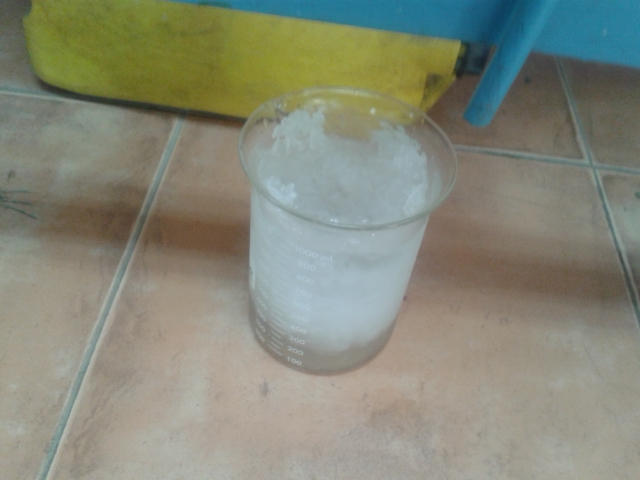
\includegraphics[scale=0.2]{agua_hielo_foto.jpg}
\caption{Envase con agua y hielo}
\label{agua_hielo_foto}
\end{center}
\end{minipage}
\hfill
\begin{minipage}[c]{.45\textwidth}
\begin{center}
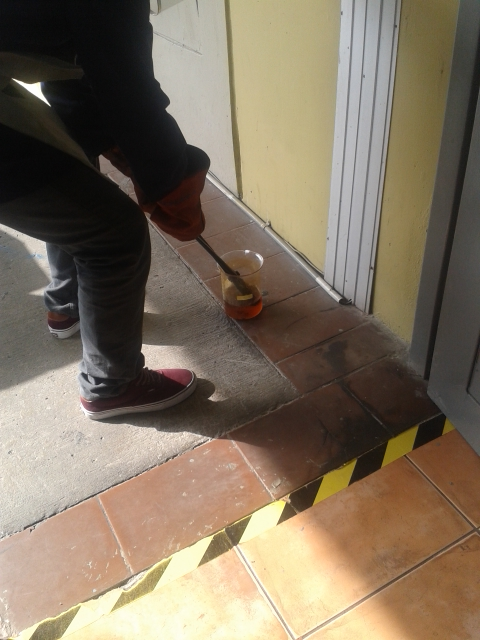
\includegraphics[scale=0.2]{practica_aceite.jpg}
\caption{Enfriamiento en aceite}
\label{practica_aceite}
\end{center}
\end{minipage}
\hfill
\end{figure}
\newpage
\begin{figure}[h] % indico que voy a poner una figura y [h] indica que la posición relativa, tambien puedo usar t = top entre otros.

\hfill
\begin{minipage}[t]{.45\textwidth}
\begin{center}
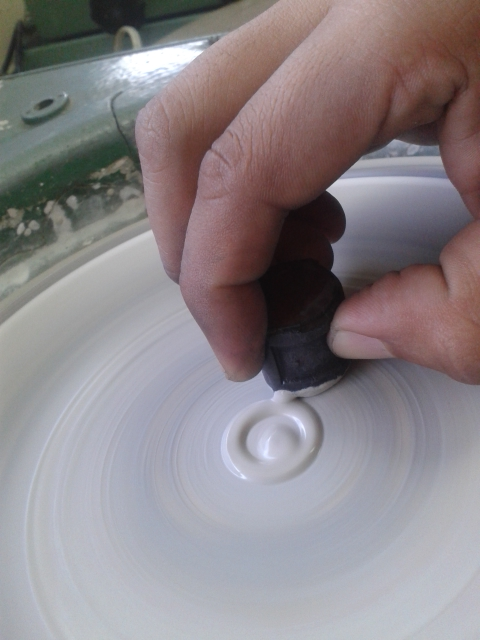
\includegraphics[scale=0.2]{pulido_fino.jpg}
\caption{Banco de lijas}
\label{pulido_fino}
\end{center}
\end{minipage}
\hfill
\begin{minipage}[t]{.45\textwidth}
\begin{center}
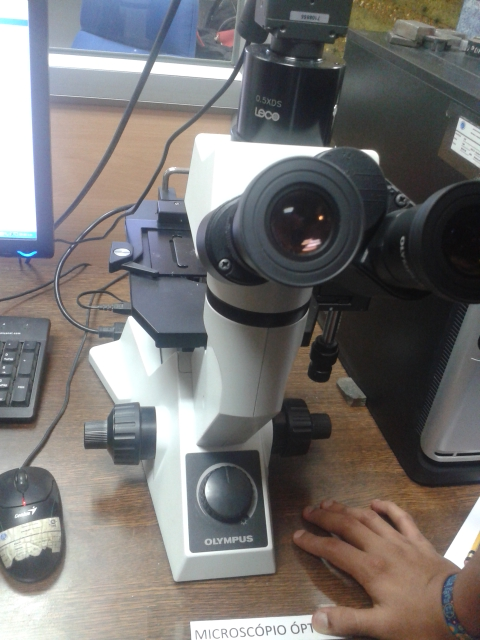
\includegraphics[scale=0.2]{microscopio_optico.jpg}
\caption{Microscopio óptico}
\label{microscopio_optico}
\end{center}
\end{minipage}
\hfill
\end{figure}

\end{document} 
